\section{Lecture 1.}
\subsection{Difference between fluid and solid.}
Perfectly elastic solid: given shear stress $ \tau $ -> finite deformations; returns to original shape if force is released.\\
Fluid: given shear stress $ \tau $ -> finite rate of deformation; further deformation stops if force is released, but there is no return to original shape (unless an opposite force is applied).

\subsection{Definition of shear stress.}
Consider body of fluid with small rectangular element of fluid within it.\\
Newton's second law: $ \text{force} \ = \ \text{change of momentum} $.\\
Consider shear stress either as force over area or flux of momentum.
\begin{align*}
	\tau_{yx}, & \ \text{where force in $ x $-direction acts on a surface of constant $ y $.} \\
	\tau_{yx}, & \ \text{where flux of $ x $-momentum is in $ y $-direction.}
\end{align*}
\begin{figure}[H]
	\centering
	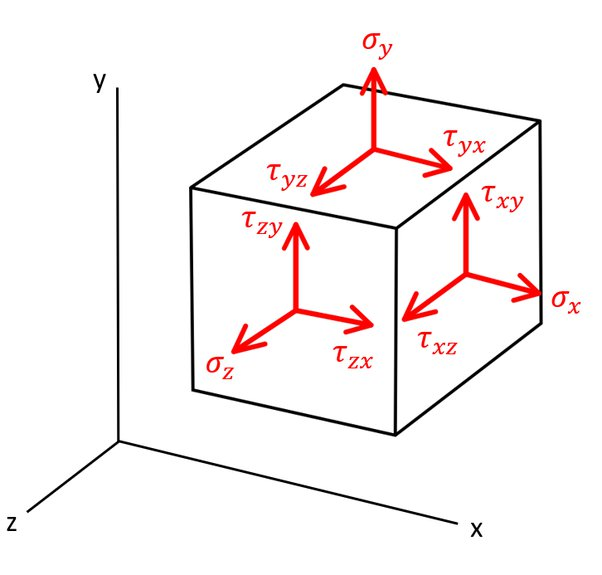
\includegraphics[width=0.1\textwidth]{shear-cube}
\end{figure}

\subsection{Newton's "law" of viscosity.}
\begin{align*}
	F/A       & = -\mu(\Delta v_x / \Delta y) = -\mu((0-v)/(y-0)) = \mu(v/y) \\
	\tau_{yx} & = -\mu(\d v_x/\d y)                                          \\
	\mu       & \equiv \ \text{viscosity of "Newtonian fluids"}              \\
	\nu       & = \ \text{Kinematic viscosity} \ \mu/\rho
\end{align*}
\begin{figure}[H]
	\centering
	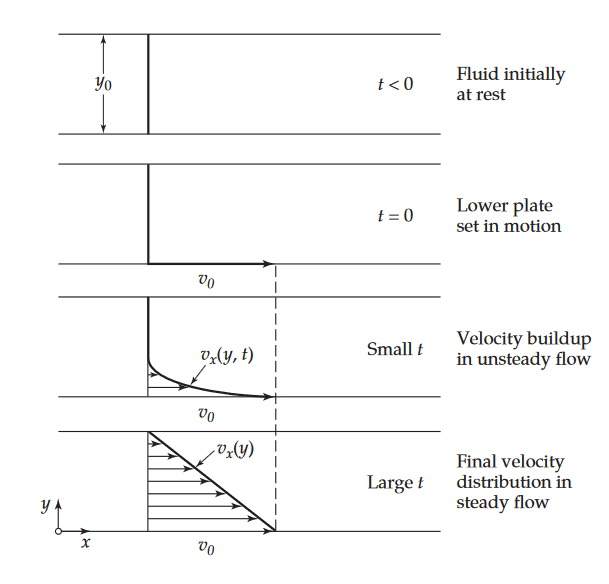
\includegraphics[width=0.25\textwidth]{newtons-law}
	\caption{BSLK Fig. 1.1-1.}
\end{figure}
Newtonian fluids are gases and simple liquids.

\subsection{Molecular origins of Newtonian viscosity.}
Consider simplest case: ideal gas, small molecules.
\begin{figure}[H]
	\centering
	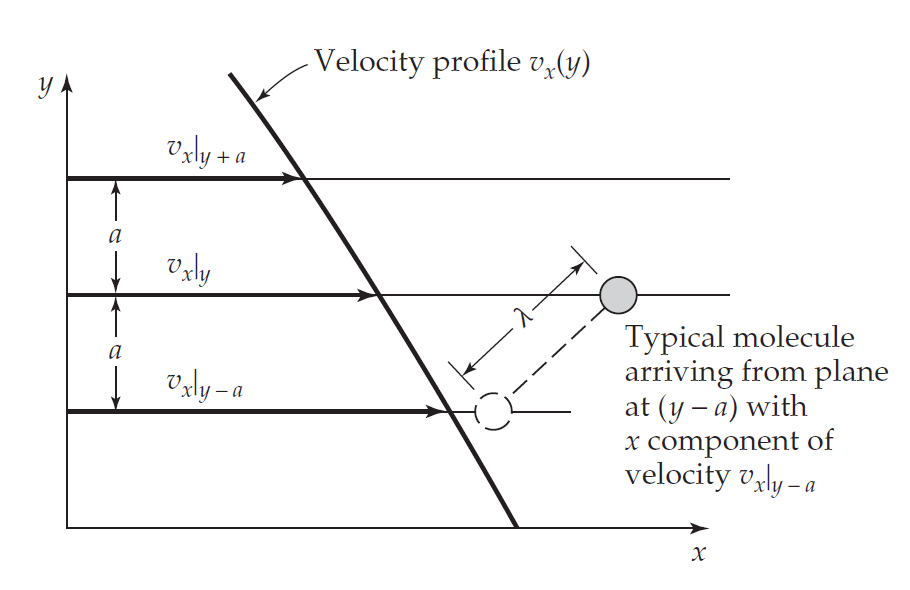
\includegraphics[width=0.2\textwidth]{molecular-origin}
	\caption{BSLK Fig. 1.6-1.}
\end{figure}
Molecules cross streamlines in random motions; they take their momentum with them when they cross.\\
Exchange of molecules between streamlines, on average, transfers momentum from fast streamlines to slow ones.\\
This momentum is transfer is the origin of "viscosity" in ideal gases (situation is more complicated in liquids).\\
In each exchange
\begin{itemize}
	\item distance is short and
	\item amount of momentum transferred is small (though there are many exchanges per unit volume per unit time)
\end{itemize}
Infinite parallel plates are impossible, so use concentric cylinders to measure viscosity.\\
If $\text{gap width}\to0$, the gap approximates planar geometry.\\
If $\text{gap width}\not\to0$, correction factors are needed.\\
This is the idea behind the Fann viscometer.

\subsection{Magnitudes of viscosity $\mu$.}
\begin{align*}
	\text{Crude oils} >> \text{Water} >> \text{Gases}
\end{align*}
Pure liquids:
\begin{itemize}
	\item $\mu$ decreases as temperature increases.
	\item $\mu$ relatively independent of pressure.
\end{itemize}
Gases at low pressures:
\begin{itemize}
	\item $\mu$ increases as temperature increases.
	\item $\mu$ independent of pressure.
\end{itemize}
Gases in or near critical region:
\begin{itemize}
	\item Trends of $\mu$ with $T$ and $P$ are complex.
\end{itemize}
Crude oils with dissolved gas:
\begin{itemize}
	\item Dissolved gas reduces $\mu$ of oil.
	\item $\mu$ decreases as $P$ decreases, until bubble point reached.
	\item $\mu$ increases as $P$ decreases further, as gas leaves solution.
\end{itemize}
\begin{figure}[H]
	\centering
	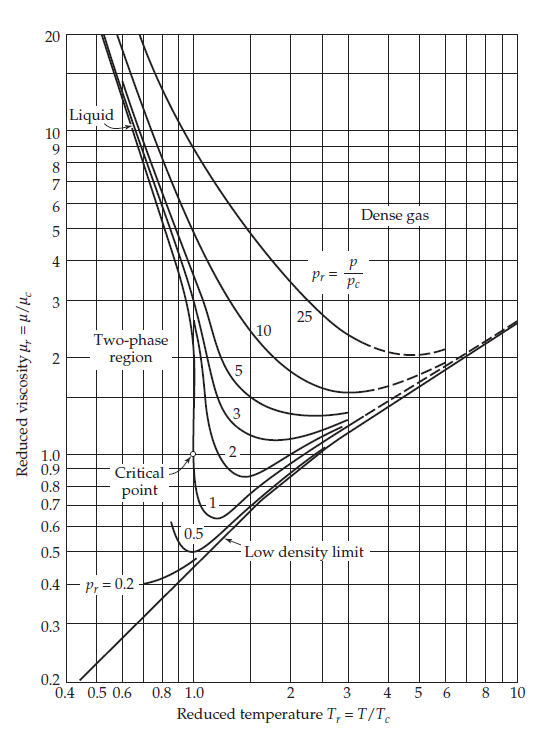
\includegraphics[width=0.15\textwidth]{reduced-viscosity}
	\caption{BSLK Fig. 1.5-1.}
\end{figure}

\subsection{Non-Newtonian fluids.}
Fluids that sometimes behave like solids: Bingham plastic.\\
Fluids that e.g. have low viscosity near well, but high viscosity away from the well: (shear-thinning) power-law fluid.\\
Recall for Newtonian fluids $\tau_{yx}=-\mu(\d v_x/\d y)$.
\begin{figure}[H]
	\centering
	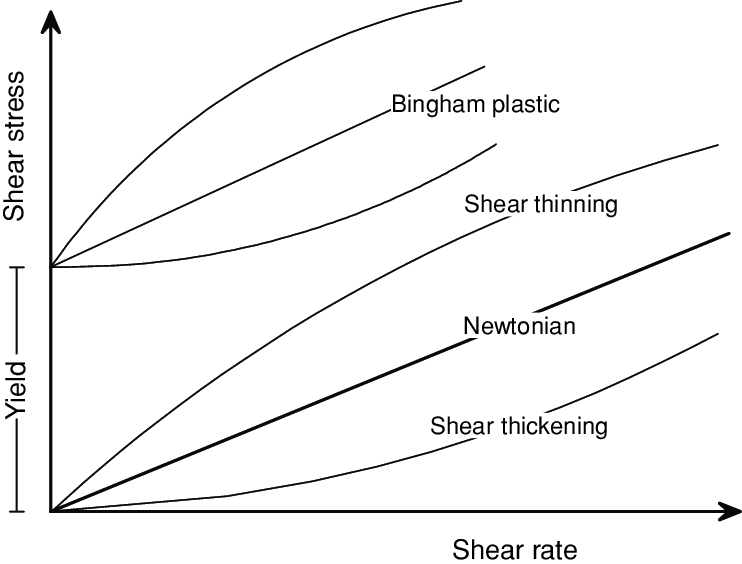
\includegraphics[width=0.2\textwidth]{fluid-types}
\end{figure}

\subsection{Bingham plastics.}
Bingham plastics are described by the following equations.
\[
	\begin{cases}
		\begin{aligned}
			\tau_{yx}           & =-\mu_0\frac{\d v_x}{\d y}+\tau_0 & \ \text{for} \ \tau_{yx}\geq\tau_0            \\
			\frac{\d v_x}{\d y} & =0                                & \ \text{for} \ -\tau_0\leq\tau_{yx}\leq\tau_0 \\
			\tau_{yx}           & =-\mu_0\frac{\d v_x}{\d y}-\tau_0 & \ \text{for} \ \tau_{yx}\geq\-\tau_0
		\end{aligned}
	\end{cases}
\]
$\mu_0$ (the slope) is sometimes called "plastic viscosity", which is not the same as (Newtonian) viscosity.\\
$\tau_0$ is the (critical) yield stress or "yield point". When $\tau_0\to0$, a Bingham plastic approaches a Newtonian fluid.

\subsection{Power-law (Ostwald-de Waele) fluids.}
Power-law fluids are described by the following equation.
\begin{align*}
	\tau_{yx}=-m\abs{\frac{\d v_x}{\d y}}^{n-1}\frac{\d v_x}{\d y}
\end{align*}
$m$ is sometimes called the "consistency index".\\
$n$ is called the "power-law index":
\begin{itemize}
	\item if $n=1$: Newtonian fluid with $m=\mu$.
	\item if $n<1$: "shear-thinning"/"pseudoplastic" where greater shear stress $\tau_{yx}\to$ much greater shear rate $\abs{\frac{\d v_x}{\d y}}$.
	\item if $n>1$: "shear-thickening/"dilatant" where greater shear stress $\tau_{yx}\to$ little increase in shear rate $\abs{\frac{\d v_x}{\d y}}$.
\end{itemize}

\section{Lecture 2.}
\subsection{Effective viscosity of non-Newtonian fluids.}
The "effective/apparent viscosity" of a non-Newtonian fluid is the viscosity of a hypothetical Newtonian fluid that would give the same result as the real fluid does in the same situation.\\
The "effective viscosity" of a non-Newtonian fluid in shear flow between parallel plates is the viscosity of a hypothetical Newtonian fluid that would give the same $\tau_{yx}$ as the real fluid does at the same $(-\d v_x/\d y)$.
\begin{figure}[H]
	\centering
	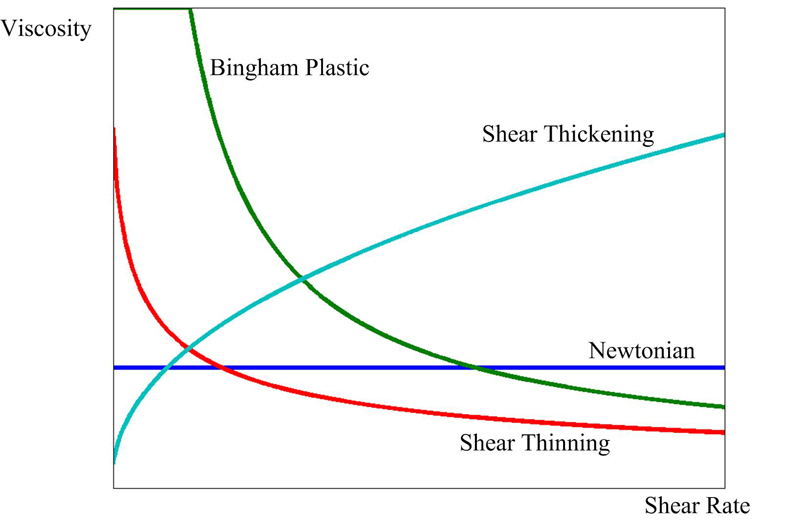
\includegraphics[width=0.25\textwidth]{viscosity-various-fluids}
\end{figure}

\subsection{Shell momentum balances.}
\begin{align*}
	\begin{pmatrix}\text{rate of momentum} \\ \text{in by convection}\end{pmatrix}
	 & -\begin{pmatrix}\text{rate of momentum} \\ \text{out by convection}\end{pmatrix}                \\
	+\begin{pmatrix}\text{rate of momentum} \\ \text{in by shear force}\end{pmatrix}
	 & -\begin{pmatrix}\text{rate of momentum} \\ \text{out by shear force}\end{pmatrix}               \\
	+\begin{pmatrix}\text{body forces (gravity)} \\ \text{acting on fluid}\end{pmatrix}
	 & =\begin{pmatrix}\text{accumulation of} \\ \text{momentum} \\ \text{(acceleration)}\end{pmatrix}
\end{align*}
First four terms: momentum crossing boundaries.\\
Last two terms: within system volume (boundaries).\\
Accumulation of momentum is zero at steady state.

\subsection{Shell momentum balance procedure.}
\textit{BSLK §2.1.}
\begin{enumerate}
	\item Select coordinate system, define control volume (boundaries either $\parallel$ or $\bot$ to velocity and thin in any direction in which velocity varies).
	\item State boundary conditions.*
	\item Perform momentum balance.**
	\item Thickness $\to0$ (gives differential equation for $\tau$).
	      \begin{enumerate}
		      \item (optional) solve differential equation for $\tau$, apply boundary condition if boundary condition applies to $\tau$ alone.
	      \end{enumerate}
	\item Relate $\tau$ to $\d v/\d x$ (apply constitutive equation).
	\item Solve differential equation for $v$, apply boundary conditions.
\end{enumerate}
*\textbf{Boundary conditions}:
\begin{enumerate}
	\item Specify $v$ at solid surface.
	      \begin{enumerate}
		      \item fluid $v$ is equal to solid velocity at solid wall.
	      \end{enumerate}
	\item Specify $\tau$ at fluid surface.
	      \begin{enumerate}
		      \item in liquid, $\tau=0$ at gas interface.
		      \item $\tau$, $v$ continuous across liquid-liquid interface.
	      \end{enumerate}
	\item $\tau$, $v$ not infinite anywhere in region of interest.
\end{enumerate}
**\textbf{Elements of momentum balance}:\\
Momentum flux ($\propto$ area), called "$\phi$" tensor.
\begin{enumerate}
	\item Convection of momentum through surface.
	\item Shear stress $\tau$ on surface ("molecular transport of momentum").
	\item Pressure pressing inward on surface.
\end{enumerate}
Momentum "generation" or "source" ($\propto$ volume).
\begin{enumerate}
	\setcounter{enumi}{3}
	\item Body forces within volume.
\end{enumerate}
Momentum accumulation ($\propto$ volume) (not a steady state!).
\begin{enumerate}
	\setcounter{enumi}{4}
	\item Acceleration of system mass - $\p(\rho v)/\p t$.
\end{enumerate}

\subsection{Four aspects can vary from one problem to another.}
\begin{itemize}
	\item Geometry (coordinate system).
	\item Elements in momentum balance.
	\item Constitutive equation (relation between $\tau$ and $\frac{\d v_x}{\d y}$).
	\item Boundary conditions.
\end{itemize}

\section{Lecture 3.}